\documentclass[]{dsadokumentation}

% Extra packages / definitions
\usepackage{amssymb}
\usepackage{amsthm}
\usepackage{algorithm}
\usepackage[noend]{algpseudocode}
\usepackage{wrapfig}



% Bibliography
\addbibresource{kurs4.2.bib}

% Custom Commands / definitions
\setcounter{chapter}{1}
\newcommand\myacademy{Wolfsberg 2022}


\begin{document}
\kurs{Die Theorie der Information}{Wie aus Daten Bilder werden}{example-image-a}

\section{Eigenwertproblem}
\sectionauthor{Lara Müller, Chuyang Wang}

\subsection{Definitionen}\label{k4.2.eigen.def}

Ein Eigenvektor ist der Vektor, welcher nach Anwendung einer Matrix immer auf einem Vielfachen von sich selbst liegt. 
Formal werden die Eigenvektoren einer quadratischen Matrix $A \in \mathbb{R}^{x \times x}$ definiert als $\vec{v} \in \mathbb{R}^{x}, \vec{v} \neq \vec{0}$, mit denen $A \cdot \vec{v} = \lambda \cdot \vec{v}$ erfüllt ist. Man nennt das Skalar $\lambda$ den zu $\vec{v}$ zugehörigen Eigenwert. 

Durch Äquivalenzumformung erhält man

\begin{equation}
  \label{k4.2.eigen.def.lgs}
  \begin{aligned}
    && A \cdot \vec{v} &= \lambda \cdot \vec{v} && \\
    &\Leftrightarrow& A \cdot \vec{v} &= \lambda E \cdot \vec{v} &\text{mit } \vec{v} = E\vec{v}& \\
    &\Leftrightarrow& (A - \lambda E) \cdot \vec{v} &= 0 && \\
    &\Leftrightarrow& B\vec{x} &= 0  \quad \quad &\text{mit } B = (A - \lambda E)&  \\ 
  \end{aligned}
\end{equation}

Die \textit{Determinante} einer Matrix ist ein skalarer Wert, welche die Eigenschaft dieser Matrix beschreibt. Dieses lineare Gleichungssystem \cref{k4.2.eigen.def.lgs} hat erst dann nicht-triviale Lösungen ($\vec{x} = 0$), wenn die Determinante von $B$ gleich $0$ ist. Also gilt $\det (B) = \det (A - \lambda E) = 0$. 

Bei dem Eigenwertproblem gilt es, diese Vektoren sowie die zugehörigen Eigenwerte zu finden. 


\subsection{Das charakteristische Polynom}

Im Allgemeinen wird das charakteristische Polynom definiert als $\chi_A (\lambda) = \det(A - \lambda E)$. Aus \cref{k4.2.eigen.def} folgt, dass man die Nullstellen dieses Polynoms finden muss, um den Eigenwert zu berechnen. 

Betrachtet man nun beispielsweise das Problem in 2D. Sei $A = \begin{pmatrix}
  a & b \\
  c & d
\end{pmatrix}$, so gilt

\begin{equation}
  \label{k4.2.eigen.charac.2d}
  \begin{aligned}
    0  
    &= \chi_A (\lambda) \\
    &= \det(A - \lambda E) \\
    &= \det \begin{pmatrix}
      a - \lambda & b \\
      c & d-\lambda
    \end{pmatrix} \\
    &= (a - \lambda) \cdot (d - \lambda) - c \cdot b
  \end{aligned}
\end{equation}

Eine allgemeine Lösung für \cref{k4.2.eigen.charac.2d} kann dann mithilfe der pq-Formel berechnet werden:

\begin{equation}
  \begin{aligned}
    \lambda = \frac{a+d}{2} \pm \sqrt{\Big(\frac{(a+d)}{2}\Big)^2-ad+cb} 
  \end{aligned}
\end{equation}


\subsection{Power Iteration}\label{k4.2.eigen.powerit}

Für $2 \times 2$ Matrizen lässt sich das Eigenwertproblem relativ gut lösen, da es eine allgemeine Formel (vgl. pq-Formel / abc-Formel) für das charakteristische Polynom existiert. Ab dem 5. Grad wird es jedoch unmöglich, eine allgemeine Formel herzuleiten \parencite{k4.2.ramond}. % Abel Ruffini Theorem 
Mit dem Power-Iteration-Algorithmus versucht man, eine Annäherung an den höchsten Eigenwert zu berechnen. Der iterative Algorithmus wählt am Anfang einen willkürlichen Wert für $b_0 \in \mathbb{R}^n$. Bei jeder Iteration aktualisiert man diesen Vektor $b$ wie folgt: 

\begin{equation}
  \begin{aligned}
    b_{k+1} = \frac{Ab_k}{\left\lVert Ab_k \right\rVert }
  \end{aligned}
\end{equation}

Nach ausreichenden Iterationen kann man den größten Eigenwert $\lambda$ berechnen, indem die Gleichung $B b_{k} = \lambda b_{k}$ nach $\lambda$ auflöst wird. 


\subsection{Anwendungen}

Eigenwerte und Eigenvektoren sind wichtige Werkzeuge für viele mathematische Rechnungen und Beweise. Ein Beispiel dafür ist die Drehung durch eine Matrix: Wenn die Matrix $A$ eine Drehung um einen bestimmten Winkel beschreibt, dann ist der Eigenvektor die Drehachse, da seine Richtung durch die Drehung nicht verändert wird. 

\section{Cox's Theorem}
\sectionauthor{Mara Germann, Patricia Hackl}
Wie berechnet man die Wahscheinlichkeit eines Ereignisses, dem ein anderes Ereignis zu Grunde liegt? Um diese Frage zu beantworten, bedarf es der Wahrscheinlichkeitsrechnung. Das Cox's Theorem ist die logische Grundlage für diese.


Beim Cox's Theorem wird die Wahrscheinlichkeitsrechnung aus  der Logik hergeleitet. Im Grenzfall für absolute Sicherheit für das Eintreten beziehungsweise Nichteintreten von Ereignissen geht die Wahrscheinlichkeitsrechnung in wahr/falsch Aussagen über. Mit Cox's Theorem entsteht eine in sich konsistente (einheitliche) Theorie für die Wahrscheinlichkeitsrechnung.
Aus dem Cox's Theorem lässt sich herleiten, dass man Wahscheinlichkeiten als Grad der Plausibilität interpretieren kann. Wir werden später sehen, dass die Plausibilität der Wahrscheinlichkeit entspricht.
Das Cox's Theorem beruht auf 3 Axiomen, die die Begründung der Bayes'schen Wahrscheinlichkeitsrechnung sind.

{
\begin{itemize}
 \item[(1.)] Der \textbf{Grad der Plausibilität} eines Ereignisses $\{b|a\}$ wird als \textbf {reelle Zahl} dargestellt. Für hohe Plausibilitäten werden hohe Zahlenwerte gewählt. Dies ermöglicht den \textbf {universellen} Vergleich voneinander unabhängiger Plausibilitäten.
 
 \item[(2.)] Sinnvolle Ergebnisse werden unter qualitativem Miteinbezug des \textbf {Verstandes} und durch logische Schlussfolgerungen erzielt.
 \item[(3.)] Es müssen \textbf {alle }verfügbaren Informationen miteinbezogen werden. An die Schlussfolgerungen wird die Anforderung der \textbf {Konsistenz }gestellt, sodass alle Sätze, die gleiches Wissen vermitteln auf gleiche Plausibilitäten hinführen müssen.
\end{itemize}
}
Aus den Axiomen ergeben sich die Produktregel und die Summenregel für Wahrscheinlichkeiten, wobei $A$, $B$ und $C$ drei Ereignisse sind.

\subparagraph{Produktregel}

Die Plausibilität $w$ des Eintretens der Ereignisse $B$ und $C$ unter der Bedingung, dass $A$ wahr ist $w(BC|A)$, 
entspricht der Plausibilität des Eintretens von $B$ unter der Bedingung, dass $A$ eingetreten ist $w(B|A)$, 
multipliziert mit der Plausibilität des Eintretens von $C$ unter der Bedingung, dass $AB$ wahr ist $w(c|AB)$:

\begin {displaymath}
w(\{BC|A\})=w(\{B|A\})\cdot w(\{C|AB\}) .
\end{displaymath}

\noindent Die Produktregel kann auf bedingte Wahrscheinlichkeiten übertragen werden:
\begin {displaymath}
P(B \wedge C|A) = P(B|A)\cdot P(C|AB).
\end{displaymath}
Unter $P(B \wedge C|A)$ versteht man die Wahrscheinlichkeit für $B$ und $C$ unter der Bedingung $A$.

Cox's Theorem erklärt zudem, warum 1 für die Wahrheit eines Ereignisses und 0 für die Unmöglichkeit eines Ereignisses stehen.

\subparagraph{Summenregel}
\begin{displaymath}
w_{ges}=w(\{B|A\}) + w(\{\bar{B}|A\})= 1 
\end{displaymath}

Die Gesamtplausibilität unter der Bedingung $A$ ist die Plausibilität von $B$ unter der Bedingung $A$ 
und die Plausibilität des Gegenereignisses von $B$ ebenfalls unter der Bedingung $A$. Die Summe der beiden Wahrscheinlichkeiten ist 1.

                                                                                  
Cox's Theorem liefert eine Herleitung für die Wahrscheinlichkeitsrechnung aus einfachen Axiomen. Es verbindet die Logik mit der Wahrscheinlichkeitsrechnung

\section{Wahrscheinlichkeitstheorie}
\sectionauthor{Mara Germann, Patricia Hackl}

Die Bayes'sche Statistik beruht auf bedingten Wahrscheinlichkeiten. Darunter versteht man die Wahrscheinlichkeit, dass ein bestimmtes Ereignis $B$ eintritt, unter der Bedingung, dass ein Ereignis $A$ bereits eingetreten ist.
\begin{displaymath}
P(B|A) = \frac{P(A \wedge B)}{P(A)} = \frac{P(B|A)\cdot P(A)}{P(B)}
\end{displaymath}
Obige Gleichung wird auch Satz von Bayes genannt. Bei unendlich vielen Ereignissen kann nicht jedem Ereignis eine bestimmte Wahrscheinlichkeit zugeordnet werden. Daher gibt man die Wahrscheinlichkeitsdichte an. Weil alle Wahrscheinlichkeiten in Summe 1 ergeben müssen, gilt für die Fläche unter der gesamten Funktion, wobei x alle möglichen Ereignisse beschreibt:
\begin{displaymath}
\int_{- \infty }^ {+ \infty} P(x) \,\mbox{d}x = 1.
\end{displaymath}

 Die Hintergrundinformation $I$ definiert das Modell, in dem wir arbeiten. Man gewinnt durch ein Experiment die Daten $d$. $P(s|I)$ beschreibt die Wahrscheinlichkeitsverteilung des Parameters $s$ des Modells. Nach dem Satz von Bayes gilt:
\begin{displaymath}
P(s|d,I) = \frac{P(d|s,I)\cdot P(s|I)}{P(d|I)}
\end{displaymath}

\begin{itemize}
 \item $P(s|I)$ gibt die Wahrscheinlichkeitsverteilung des Parameters vor dem Einbeziehen der Daten an (Prior).
 \item $P(d|I)$ ist der Normierungsparameter (Evidenz).
 \item $P(d|s,I)$ beschreibt die Wahrscheinlichkeit für die Messdaten, mit gegebenem Prior (Likelihood).
 \item $P(s|d,I)$ gibt die Wahrscheinlichkeitsverteilung des Parameters unter Einbezug der Daten und Informationen (Posterior).
\end{itemize}

Das Experiment kann mehrfach wiederholt werden, dabei werden die Daten angepasst. So dient der Posterior bei erneuter Durchführung als Prior und wir lernen sukzessive von Daten d und aktualisieren unser Wissen über s.

\section{Lineare Abbildungen zwischen Vektorräumen}
\sectionauthor{Lara Müller, Chuyang Wang}
Der folgende Abschnitt wird sich mit den Grundlagen linearer algebraischer Berechungen befassen und in diesem Kontext lineare Abbildungen und zugehörige Vektorräume definieren.

\subsection{Grundlagen linearer Algebra}
Ein Vektorraum über dem Körper $K$ einer Zahlenmenge ist definiert als Menge $V$, die zusammen mit einer Addition, sowie einer skalaren Verfielfachung auftritt. Für die Vektoren jedes linearen Vektorraums müssen folgende grundlegende Rechenregeln gelten:
\begin{itemize}
\item Kommutativgesetz: $\vec{a} + \vec{b} = \vec{b} + \vec{a}$
\item Assoziativgesetz: $\vec{a} + \vec{b} + \vec{c} = (\vec{a} +\vec{b}) + \vec{c} = \vec{a} + (\vec{b} +\vec{c})$
\item Distributivgesetz: $\vec{a} \cdot (\vec{b} + \vec{c}) = \vec{a} \cdot \vec{b} + \vec{a} \cdot \vec{c}$
\end{itemize}

Der Gegenvektor eines Vektors $a$ ist definiert als $b = -a$, sodass gilt $a + b = 0$. Eine skalare Vervielfachung bechreibt allgemein die Multiplikation eines Vektors mit einer reellen Zahl $\lambda \in \mathbb{R}$, wodurch die Vektorlänge eines beliebigen Vektors $\vec{a}$ (hier: dreidimensional) variiert werden kann. Gilt $\lambda < 0$, so wird zudem die Richtung des Vektors umgekehrt:
\begin{center} $\vec{a} \cdot \lambda = \left(\begin{array}{c} a_1 \\ a_2 \\ a_3 \end{array}\right)\cdot \lambda=\left(\begin{array}{c} a_3 \lambda \\ a_2 \lambda \\ a_1 \lambda \end{array}\right)$ \end{center}

\subsection{Definition - Lineare Abbildungen}
Jede Darstellung, deren Additivität ebenso gegeben ist, wird als lineare Abbildung (auch: Vektorhomomorphismus) $f: V \rightarrow W$ definiert. Bezüglich der zwei $K$-Vektorräume $V$ und $W$ kann die Abbildung dementsprechend als linear bezeichnet werden, sofern gilt:
\begin{center} $f(\lambda v + \mu w)=\lambda f(v) + \mu f(w) \quad \forall \; \lambda, \mu \in K \quad \forall \; v, w \in V$ \end{center}

\subsection{Eigenschaften von Vektorräumen}
Darüber hinaus bezeichnet die Menge der Vektoren, die auf den Nullvektor $\vec{o}$ abgebildet werden, als Kern der zugehörigen linearen Abbildung. Der Kern $ker(f):= \{v \in V \; \big\vert \; f(v) \} = 0$ entspricht demnach einem Vektor aus dem Vektorraum $V$ ($ker(f) \subseteq V$), in dem auch der Nullvektor enthalten ist ($\vec{o} \in ker(f)$). Vektorräume können unendlichdimensonal sein und somit beispielsweise als reeller ($V \in \mathbb{R}$) oder komplexer ($V \in \mathbb{C}$) Vektorraum auftreten. Die jeweilige Dimension eines endlichdimensionalen Vektorraums $K^n$ kann über die zur Darstellung zwingend notwendige Mindestanzahl an Basisvektoren bestimmt werden. Es lässt sich beweisen, dass die Anzahl an Dimensionen, die mithilfe eines Vektors beschrieben werden, für jede Basis eines gegebenen Vektorraums gleich sein muss. 

\subsection{Darstellung linearer Abbildungen durch Matrizen}
Lineare Abbildungen lassen sich auch über Matrizen darstellen. Dementsprechend gilt für eine lineare Abbildung in dem zweidimensionaen Vektorraum $K^2$, der über die Basisvektoren $\vec{u}$ und $\vec{v}$ dargestellt werden kann:
\begin{center} $x \cdot \left(\begin{array}{c} u_1 \\ u_2 \end{array}\right) + y \cdot \left(\begin{array}{c} v_1 \\ v_2 \end{array}\right) = \left(\begin{array}{c} u_1 x + v_1 y \\ u_2 x + v_2 y \end{array}\right) = \left( \begin{array}{rr} u_1 & v_1 \\ u_2 & v_2 \end{array}\right) \cdot \left(\begin{array}{c} x \\ y \end{array}\right)$ \end{center}

Die resultierende $2$x$2$-Matrix beinhaltet entsprechend der Matrix-Spalten sowohl das Bild des ersten, als auch das des zweiten Basisvektors. Allgemein lassen sich lineare Abbildungen $f(\vec{x})$ über eine zugehörige Matrix A definieren:
\begin{center} $f(\vec{x}) = A \cdot \vec{x}$ \end{center}

Bei einer linearen Abbildung stellt $f(\vec{x})$ selbst auch stets wieder einen Vektorraum dar. Dabei bleiben Streckenverhältnisse und Lagebeziehungen unverändert. Im Gegensatz zur Drehung, Scherung und Projektion bei der Abbildung sind Krümmungen nicht möglich. \\

Mithilfe diesem Wissen über lineare Algebra und Abbildungen in Zusammenhang mit Vektorräumen, lassen sich lineare Abbildungen nun als strukturerhaltende Abbildungen zwischen Vektorräumen auffassen.

\section{Radioastronomie}
\sectionauthor{Constantin Burmeister, Ole Fleck}

Radioastronomie dient der Beobachtung von Ereignissen und astrophysikalischen Prozessen, welche Wellen außerhalb des Frequenzbereichs des sichtbaren Lichts aussenden. Diese Signale werden mit Radiointerferometrie nachbehandelt und zusammengefügt.

\subsection{Teleskope}

Die Radioastronomie verwendet Radioteleskope, um Daten über astrophysikalische Prozesse aufzunehmen.
Der minimal auflösbare Bildwinkel $\delta\theta$ ist abhängig von der Wellenlänge $\lambda$, welche gemessen werden soll, und dem Spiegeldurchmesser $D$ des Teleskops mit $\delta\theta\approx1,22\frac{\lambda}{D}$.
Da die Radioastronomie große Wellenlängen im $cm-km$ Bereich verwendet, sind hier auch bei Teleskopen mit großen Spiegeldurchmessern von über $100m$ nur geringe Auflösungen möglich. Zur Erhöhung der Auflösung von Teleskopen können mehrere Antennen gleichzeitig verwendet werden.

\subsection{Radiointerferometrie}
\begin{wrapfigure}{r}{5cm}
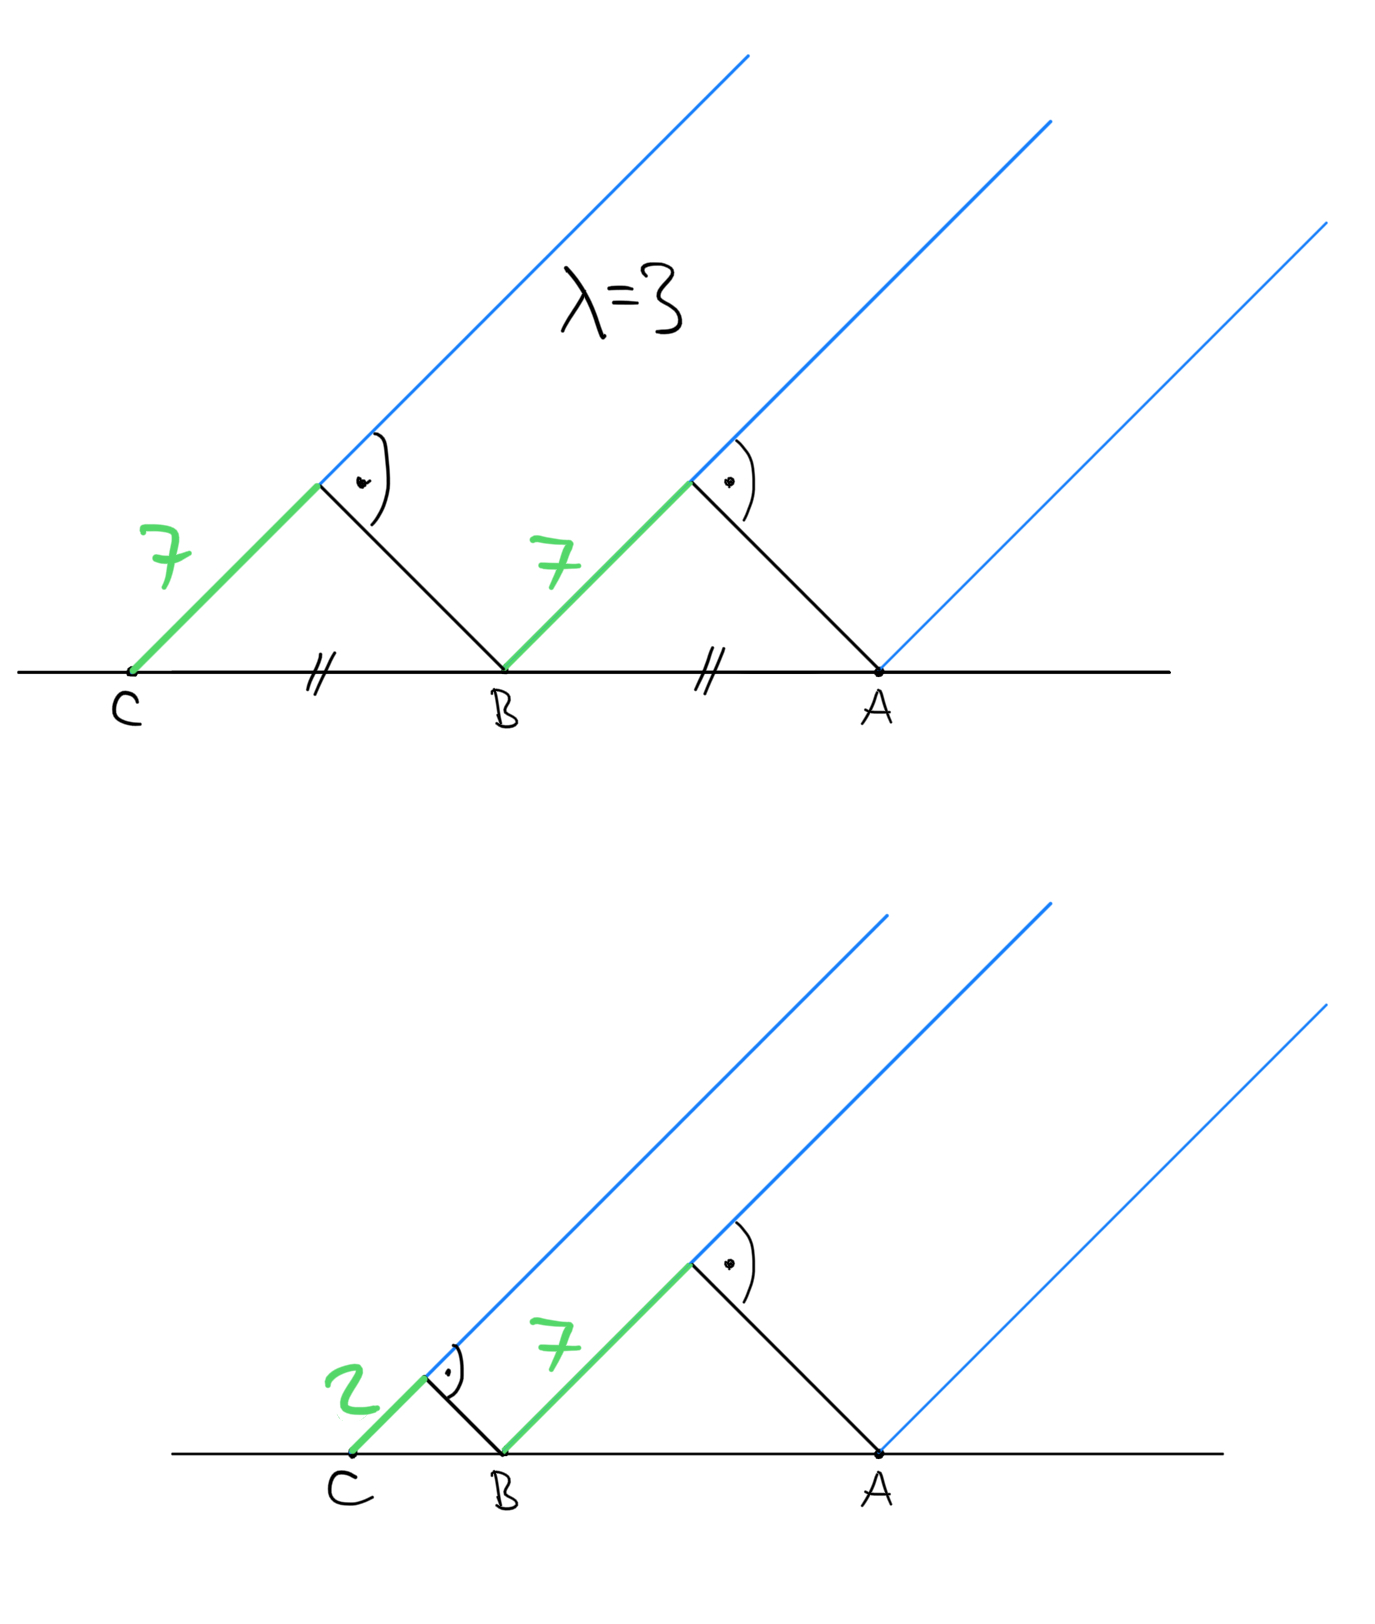
\includegraphics[width=.4\textwidth]{k4.2/baselineunterschied.png}
\caption{Gangdifferenzen von Radiowellen bei Antennenarrays}
\label{bildBaselineunterschied}
\end{wrapfigure}

Radiointerferometrie ist ein Verfahren zur Überlagerung von Radiowellen, welche von mehreren Antennen aufgezeichnet wurden, um hieraus ein Signal zu erzeugen. Dieses Signal soll dem Signal, welches von einer Antenne mit dem Spiegeldurchmesser entsprechend des Antennenabstandes erzeugt worden wäre, möglichst ähnlich sehen.

Werden mehrere Teleskope in einem Verbund synchronisiert, ist nur die Laufzeitdifferenz im Vergleich zum Wellenberg bekannt, da die einzelnen Wellenberge nicht unterschieden werden können. So können, wie im Beispiel  \ref{bildBaselineunterschied}, bei gleichen Abständen nicht zwischen den Gangdifferenzen $mod \lambda$ unterschieden werden. In diesem Beispiel ist aus den Messwerten nicht ersichtlich, ob es sich tatsächlich um $2\cdot \lambda +1$ Gangunterschied handelt, sondern jedes $x$ in $x\cdot\lambda+1$ ist möglich. Werden Antennen mit unterschiedlichen Abständen verwendet, sinkt die Anzahl der Kombinationen der Gangunterschiede, für welche sich eine solche Gleichung lösen lässt. Daher werden bei Antennengruppen möglichst unterschiedliche Abstände verwendet.

Dieses Verfahren wurde beispielsweise auch \emph{Event Horizon Telescope} verwendet. Das \emph{Event Horizon Telescope} besteht aus einer Verschaltung mehrerer Teleskope, wobei deren Abstand bis zu $10000km$ beträgt. Mit diesem Teleskop wurde das erste Foto eines Schwarzen Lochs erstellt.

Die Radiointerferometrie ist also ein essenzieller Bestandteil der Astronomie. Nur dieses Verfahren ermöglicht die Ursprungsbestimmung eines Radiowellen Signals.

\subsection{Zusammenfassung}
Die Radioastronomie erstellt mithilfe von Teleskopen und Antennenarrays Bilder des Weltraums. Die Radiointerferometrie verarbeitet das Signal der Teleskope in Bilder.

% Bibliography
\printbibliography{}
\end{document}
